\documentclass{school-22.211-notes}
\date{April  9, 2012}

\begin{document}
\maketitle

\lecture{Fission Product Poisoning}
\topic{Fission Product Chain}
\begin{figure}
  \centering
  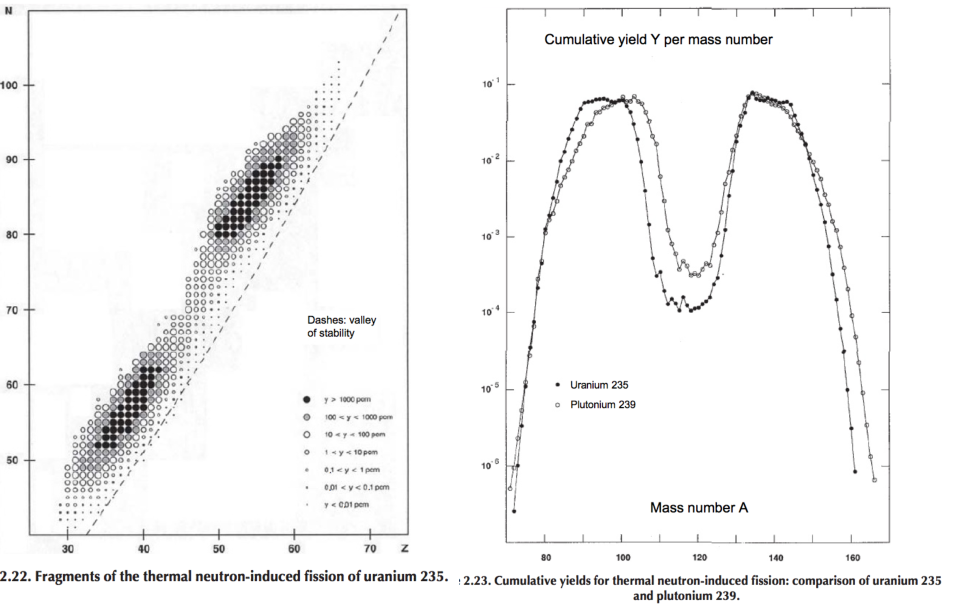
\includegraphics[width=5in]{images/dfs/fission-product-yield.png}
  \caption{Fission Product Yields, Fission Fragments}
\end{figure}

The fission products have the following properties: 
\begin{enumerate}
\item Number: almost all fissions produce precisely two fission produces per fission;
\item Unstability: most fission products are highly unstable and radidly decay to other nuclides;
\item Thermal spectrum: some fission produces have large thermal absorption cross sections, which are important for thermal spectrum reactors as in Figure~\ref{major-capture};
\item Fast spectrum: fast reactors are much less sensitive to fission products, because thermal spectrum does not matter. 
\item Distribution: contributing factors are: which species are fissioned (U235, Pu239, etc), the incident fission neutron energy, random statistical fluctuations nuclide breakup.
\end{enumerate}
\begin{figure}
  \centering
  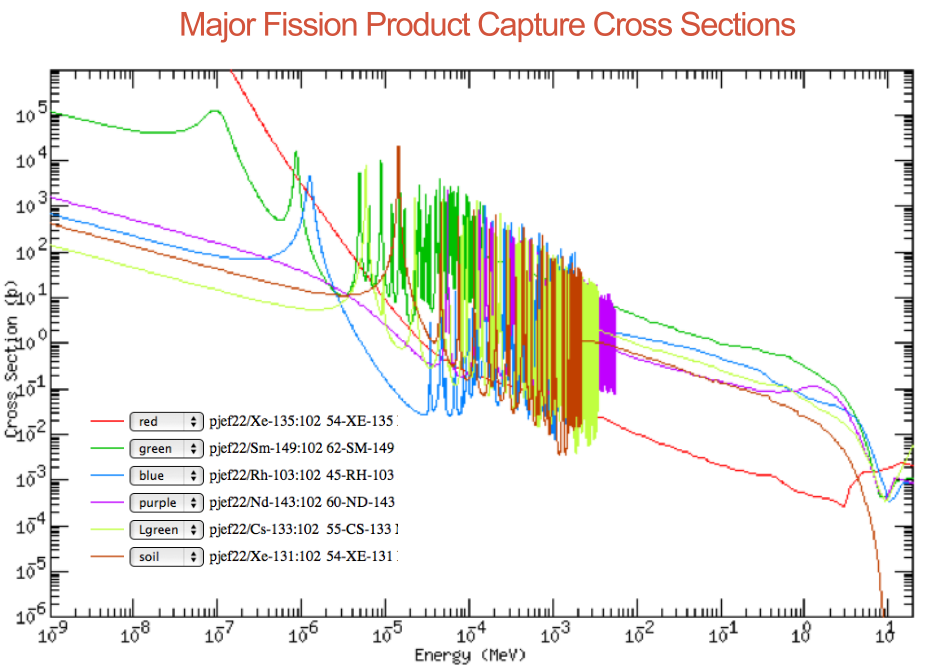
\includegraphics[width=3.5in]{images/dfs/fission-product-capture-xs.png}
  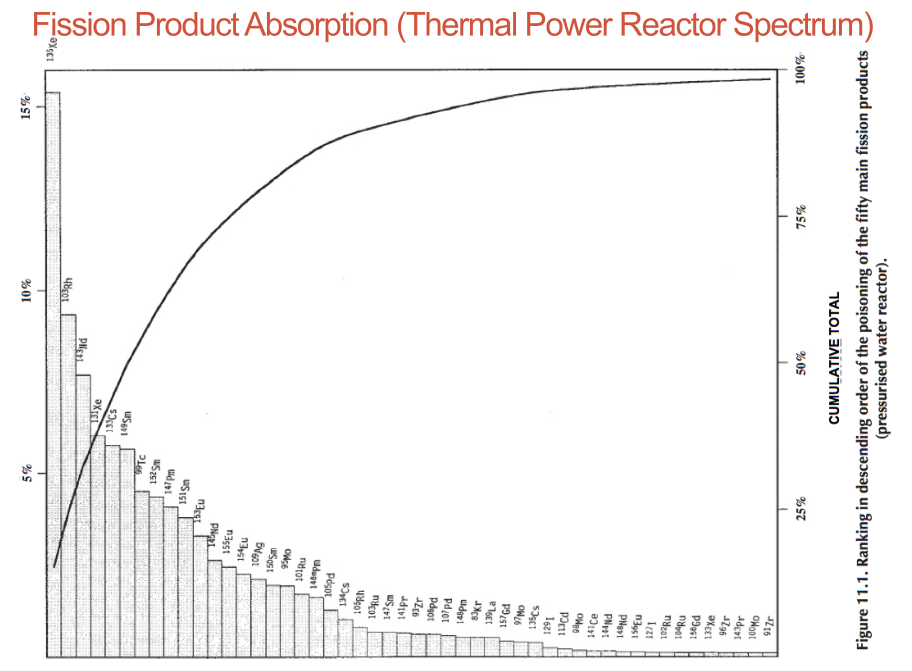
\includegraphics[width=3.5in]{images/dfs/fission-product-absorption.png}
  \caption{Major Fission Products Absorption} \label{major-capture} 
\end{figure}

\begin{figure}
  \centering
  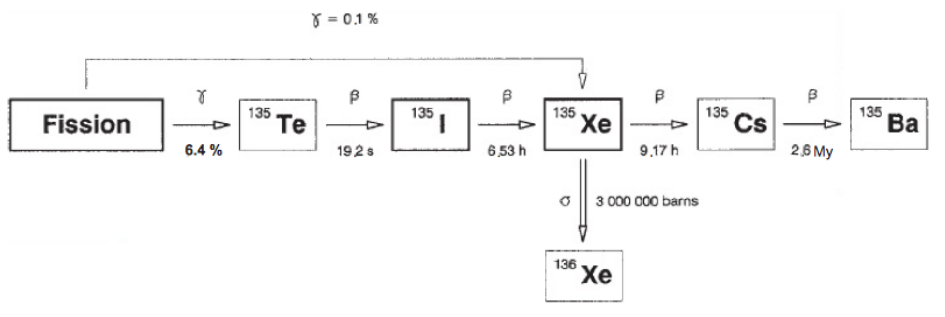
\includegraphics[width=3.5in]{images/dfs/Xe135.png}
  \caption{Xe135 Chain} \label{Xe135} 
\end{figure}

As an example, we look at the Xenon-135 Chain in Figure~\ref{Xe135}. Notice the independent fission yield is a different concept from the cumulative fission yield. Typically very rapid transitions are not followed in details when modeling reactor behavior. For instance, because Te's half-life is 19s, we can assume that \ce{^{135}I} is producted instantenously. Most of the chains are similar and are dominated by beta decays until they are stable. 

Meda-stable state: an isotope may not directly decay into a stable state; it may branch into a meda-stable state. For our purpose, we are going to take the simplified approach.



\clearpage
\topic{Nuclide Balance Equations}
\subtopic{Meaning of Nuclide Balance Equation}
\begin{figure}[ht]
  \centering
  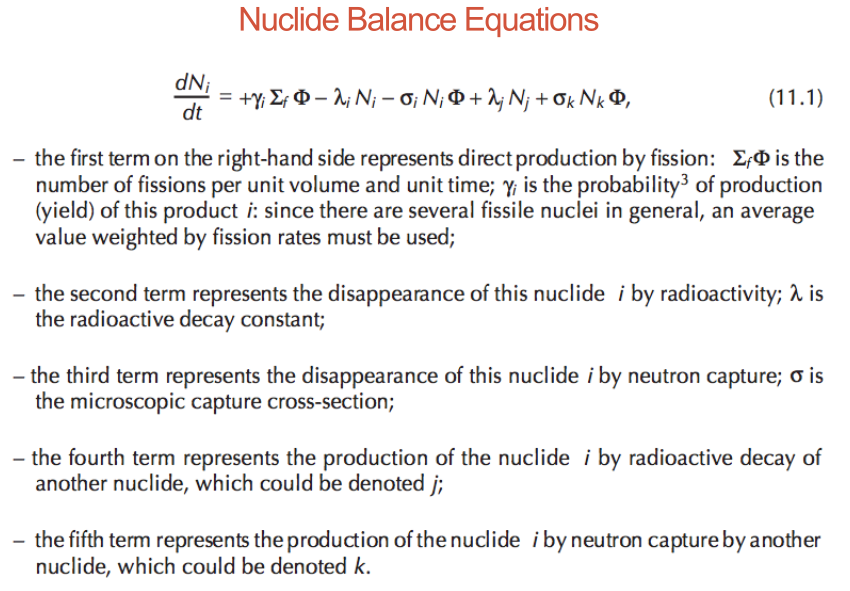
\includegraphics[width=5in]{images/dfs/nuclide-balance-equation.png}
  \caption{Nuclide Balance Equation} \label{nbe} 
\end{figure}
We discuss how to solve the nuclide depletion equation as in Figure~\ref{nbe}. 
\begin{align}
\dNdt + A(t) N(t) &= Y \\
\mbox{IF} &= e^{\int A(t) \dt} = e^{At} \\
e^{At} \dNdt + e^{At} A(t) N(t) &= e^{At} Y \\
\ddt[e^{At} N(t) ] &= e^{At} Y \\
e^{At} N(t) &= A^{-1} e^{At} Y + C 
\end{align}
Then using the particular solution that $N_0 = N(t=0$, then 
\eqn{ N_0 = A^{-1} Y + C \Rightarrow C = N_0 - A^{-1} Y } 
That is, 
\eqn{ e^{At} N(t) = A^{-1} [e^{At} Y - Y ] + N_0 }
\eqn{ \boxed{ N(t) = e^{-At} N_0 + e^{-At} A^{-1} [e^{At} Y - Y ] } }
We can also write the above differential equation into the matrix form as in Figure~\ref{depletion-matrix}. Notice we asume fission yields, cross sections, and fluxes are constant over the time interval $t_{n-1}, t_n$,
\eqn{ [N(t_n)] = e^{-[A] \Delta t_n} [N(t_{n-1})] + e^{-[A]\Delta t_n} [A]^{-1} [e^{[A] \Delta t_n} Y - Y ] }
\begin{figure}[ht]
  \centering
  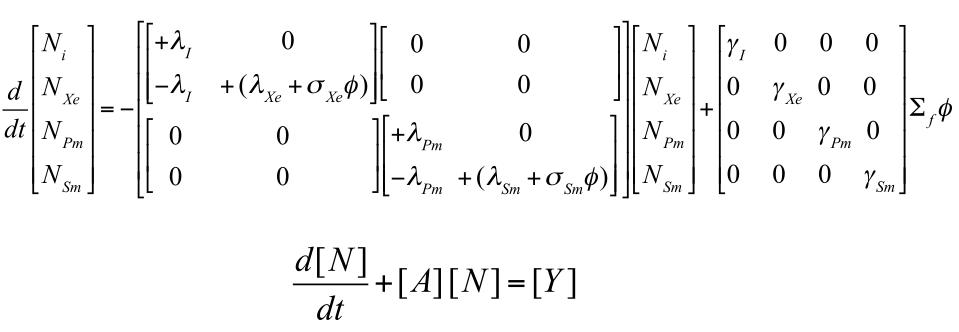
\includegraphics[width=5in]{images/dfs/depletion-matrix-form.png}
  \caption{Nuclide Depletion Equations in Matrix Form} \label{depletion-matrix} 
\end{figure}





\clearpage
\topic{Iodine/Xenon}
\begin{figure}[ht]
  \centering
  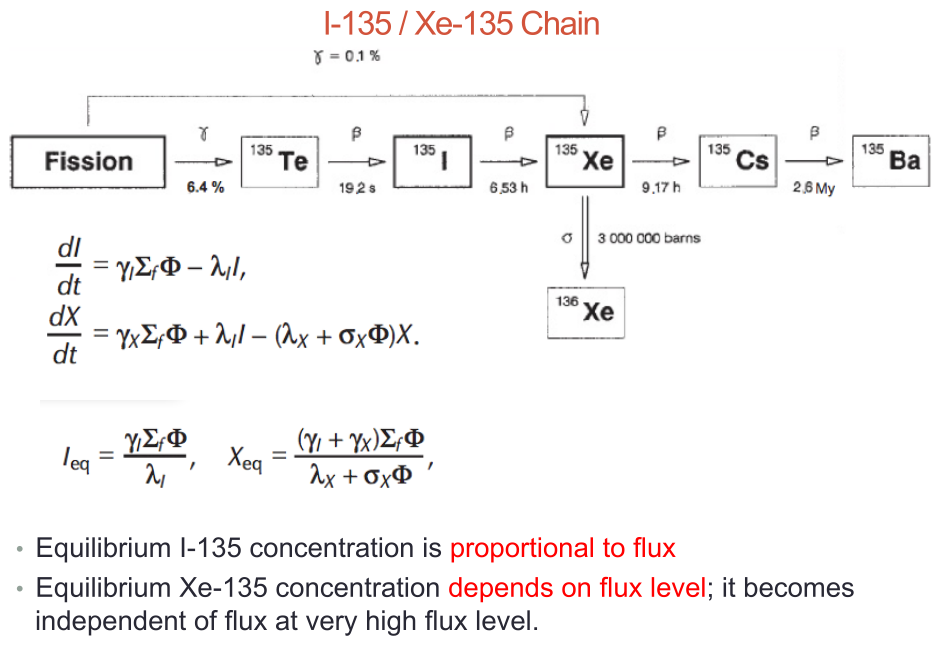
\includegraphics[width=5in]{images/dfs/I-Xe.png}
\end{figure}

\begin{table}
  \centering
  \begin{tabular}{|p{3in}|p{3in}|}\hline
    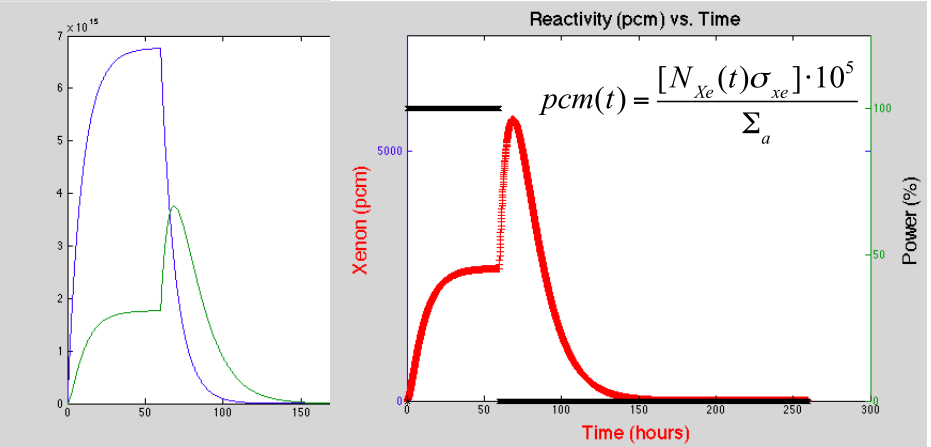
\includegraphics[width=3in]{images/dfs/I-Xe-1.png} & After startup and shutdown: Iodine increases and decreases with power; Xenon would generate a peak everytime there is a shutdown. There is a 2.5\% depress due to Xe; the higher the flux, the higher the peak is; the time of the peak is 9 hours; \\ \hline
    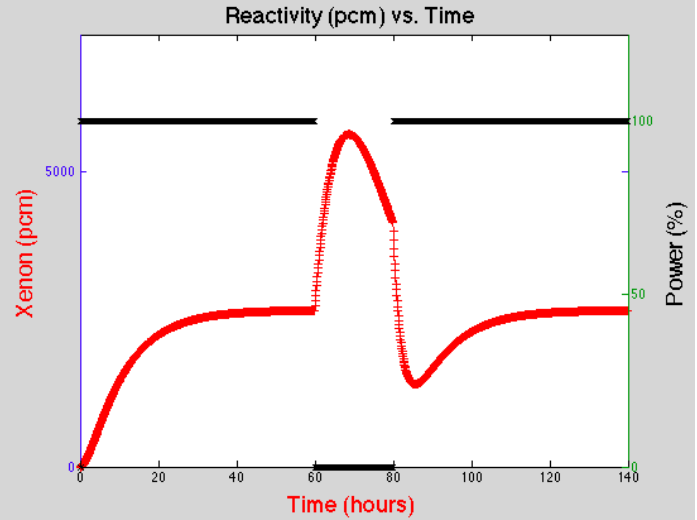
\includegraphics[width=3in]{images/dfs/I-Xe-2.png} & Xenon worth following a rapid startup after a scram: the absorption of Xenon  \\ \hline
    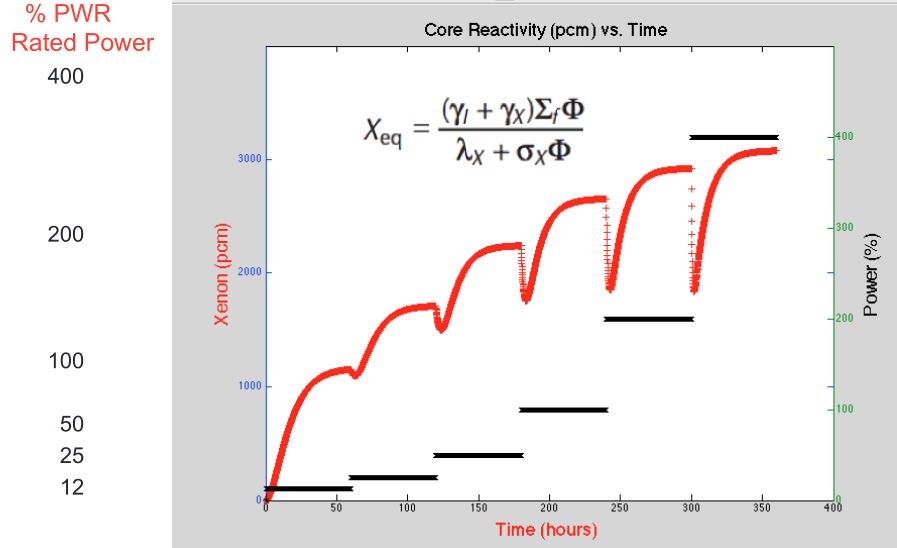
\includegraphics[width=3in]{images/dfs/I-Xe-3.png} &  Equilibrium Xenon Worth: if $\phi \to infty$, then $X_{eq}$ is independent of the flux; the flux is changing instantenously, hence the destruction rates of Xe, but the Idine decay rate has not increased to this level yet. \\ \hline
    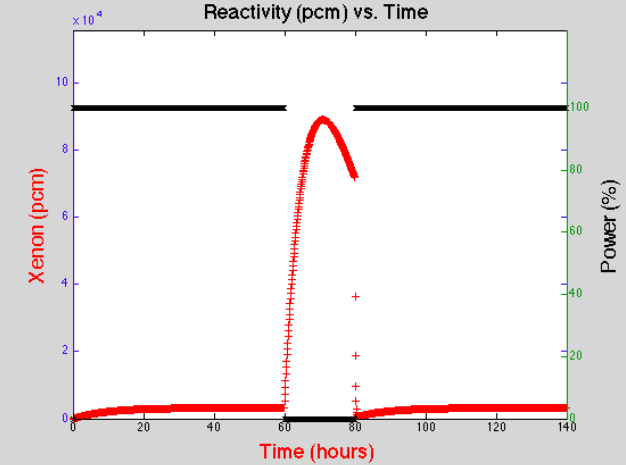
\includegraphics[width=3in]{images/dfs/I-Xe-4.png} &  Xenon for high flux reactor: you do not want to scram for a high flux reactor, because the Xenon reactivity build-up is so large; alternatively, you can start before Xenon builds up, which is pretty rare. \\ \hline
  \end{tabular}
\end{table}


\clearpage
\topic{Promethium/Samarium}
\begin{figure}[ht]
  \centering
  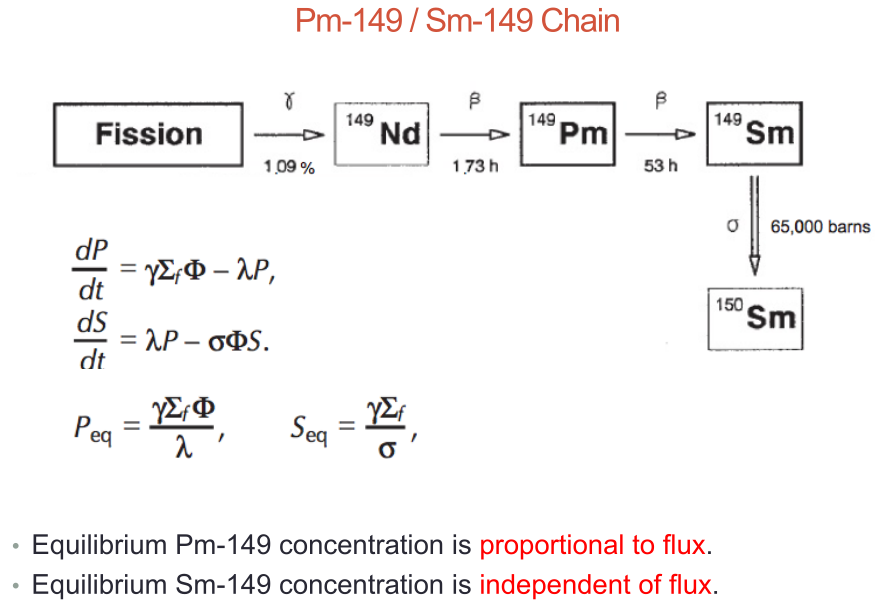
\includegraphics[width=5in]{images/dfs/Pm-Sm.png}
\end{figure}

\begin{enumerate}
\item Promethium/Samarium after starup and shutdowns: Promethium increases and decreases relative to power; Samarium comes from Promethium, but it is stable unlike Xenon. Hence once Pm burns out, Sm would not change neither. Sm peaks 200 hours after shutdown, and never decays away. 
\item Samarium worth following a refueling outage: Over-write Xenon by pulling the control rods out for a couple of days; then insert the control rods for Samarium. 
\end{enumerate}
\begin{figure}[ht]
  \centering
  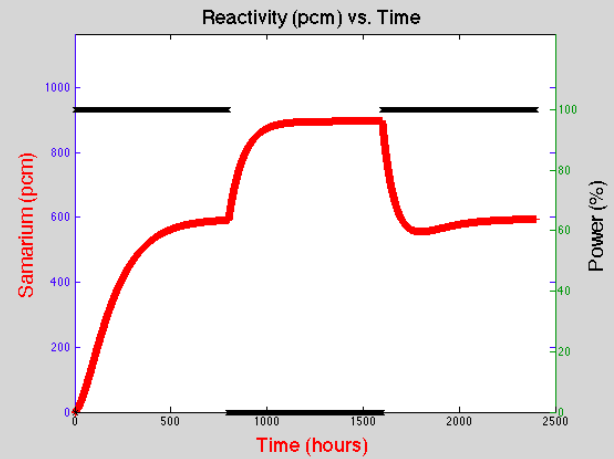
\includegraphics[width=3in]{images/dfs/Pm-Sm-1.png} 
  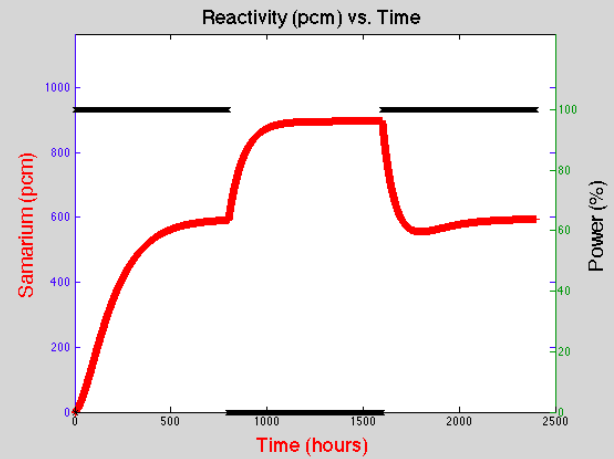
\includegraphics[width=3in]{images/dfs/Pm-Sm-2.png} 
\end{figure}



\clearpage
\topic{Spatial Xenon Oscillations}
The top and the bottom of the core are doing different things: 

Chasing Xenon, meaning placing the control rods where there are high concentration of Xenon, is wrong because we are nine hours out of sync then. 
\begin{figure}[ht]
  \centering
  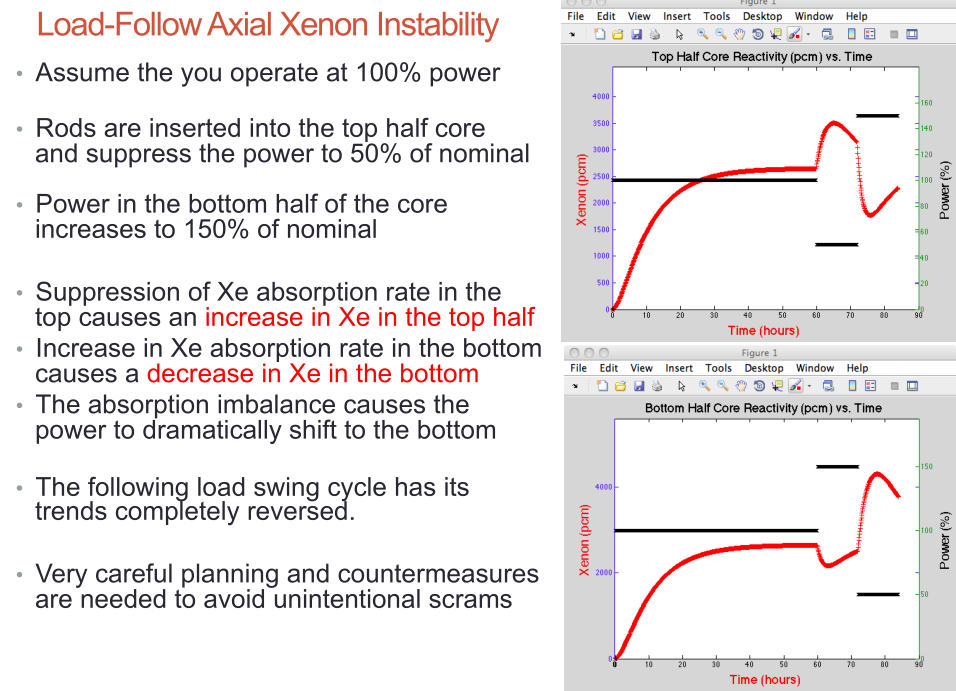
\includegraphics[width=5in]{images/dfs/axial-xenon-instability.png}
\end{figure}

\clearpage
\topic{Production Codes' Fission Product Modeling}
\begin{enumerate}
\item Point Fuel Models: ORIGEN;
\item Lattice Physics: 
  \begin{enumerate}
    \item Traditional models: 30 FPs, 2 lumped FPs (these fission products do not saturate; they increase as burnups).
    \item Latest codes: 250 FPs. 
  \end{enumerate}
\item Core Models: 
  \begin{enumerate}
    \item Traditionally: explicit I/Xe, Pm/Sm, all other FPs are resiual macros (depend on burnups);
    \item Latest codes: 
  \end{enumerate}
\end{enumerate}

Benchmark: Nd is a burnup marker term: each fission produces a fixed amount of Nd (Pu and U produces slightly different amount of Nd). Use Nd number density, from the yield, you can back out the burnups. 

Gd156 and Gd157 are important for startups when using old rods (15 years old). Once operating, we don't really care about Gd that much. 


\end{document}
